\section{Introduction}

\begin{frame}{Introduction}
    In this presentation, we will be discussing quantum channels and how they developed from classical channels. But before that, we need to define what quantum channels
    are and what they operate on. \\
    Quantum channels operate on Density Matrices, which are mathematical constructs that hold all information about a quantum state. They can be defined as:
    \begin{equation}
        \rho = \sum_{i}p_i | \psi_i \rangle \langle \psi_i |   
    \end{equation}
    where $\psi_i$ is the $i^{th}$ state occuring with probability $p_i$
\end{frame}

\begin{frame}{Introduction}
    A quantum channel acts as a linear \textit{Completely Positive Trace Preserving (CPTP)} map from one density matrix to the other. This means that the product state
    of the system and the environment stays positive throughout the transformation, and the trace remains constant. These two properties are essential for a channel to
    be physically viable and make sense in the real world.\\
    It is usually denoted with $\mathcal{N}$ and the state generated after the application of the channel on the original state is $\mathcal{N} (\rho)$.\\
    Generally, this channel is second one of the three steps that happen in the process of sending information from A to B, the others being encoding and decoding.
    These three steps have been illustrated in the following figures.
\end{frame}

\begin{frame}{Quantum channel conditions}
    Three conditions:
    \begin{description}
        \item[Linearity] {
            A quantum channel must satisfy:
            \begin{equation}
                \mathcal{N}(\alpha X_A + \beta Y_A) = \alpha \mathcal{N}(X_A) + \beta \mathcal{N}(Y_A)
            \end{equation}
            }
        \item[Complete Positivity] {
            It must have complete positivity:
            \begin{definition}[Complete Positivity]
                A linear map $\mathcal{M} : \mathcal{L}(\mathcal{H}_A) \rightarrow \mathcal{L}(\mathcal{H}_B)$
                is said to be completely positive if $id_R \otimes \mathcal{M}$ is positive map for a reference
                system $R$ of arbitrary size.
            \end{definition}
        }
        \item[Trace Preserving] {
            Channel must be trace preserving
            \begin{definition}[Trace Preservation]
                A map $\mathcal{N}$ is trace preserving if $Tr[X_A] = Tr[\mathcal{N}(X_A)]$ for all input $X_A \in \mathcal{L}(\mathcal{H}_A)$
            \end{definition}
        }
    \end{description}
\end{frame}

\begin{frame}{Choi Operator}
    \begin{definition}[Choi Operators]
        Let $\mathcal{H}_R$ and $\mathcal{H}_A$ be isomorphic Hilbert spaces, and let
        $\{| i\rangle_R \}$ and $\{|i\rangle_A \}$ be orthonormal bases for $\mathcal{H}_R$
        and $\mathcal{H}_A$, respectively. Let $\mathcal{H}_B$ be some other Hilbert space,
        and let $\mathcal{N} : \mathcal{L}(\mathcal{H}_A) \rightarrow \mathcal{L}(\mathcal{H}_B)$
        be a linear map (written also as $N_{A\rightarrow B}$). The Choi operator corresponding
        to $N_{A\rightarrow B}$ and the bases $\{| i\rangle_R \}$ and $\{|i\rangle_A \}$ is defined
        as the following operator:
        \begin{equation}
            (id_R \otimes \mathcal{N}_{A \rightarrow B})(| \Gamma \rangle\langle \Gamma |_{RA})
            = \displaystyle\sum_{i,j = 0}^{d_A-1}| i \rangle\langle j |_R \otimes \mathcal{N}_{A \rightarrow B}(| i \rangle\langle j |_A)
        \end{equation}
        where $d_A \equiv dim(\mathcal{H}_A)$ and $| \Gamma \rangle_{RA}$ is the unnormalized maximally entangled vector:
        \begin{equation}
            | \Gamma \rangle_{RA} \equiv \displaystyle\sum_{i=0}^{d_A - 1} | i \rangle_R \otimes | i \rangle_A
        \end{equation}
    \end{definition}
\end{frame}

\begin{frame}
    \begin{figure}
        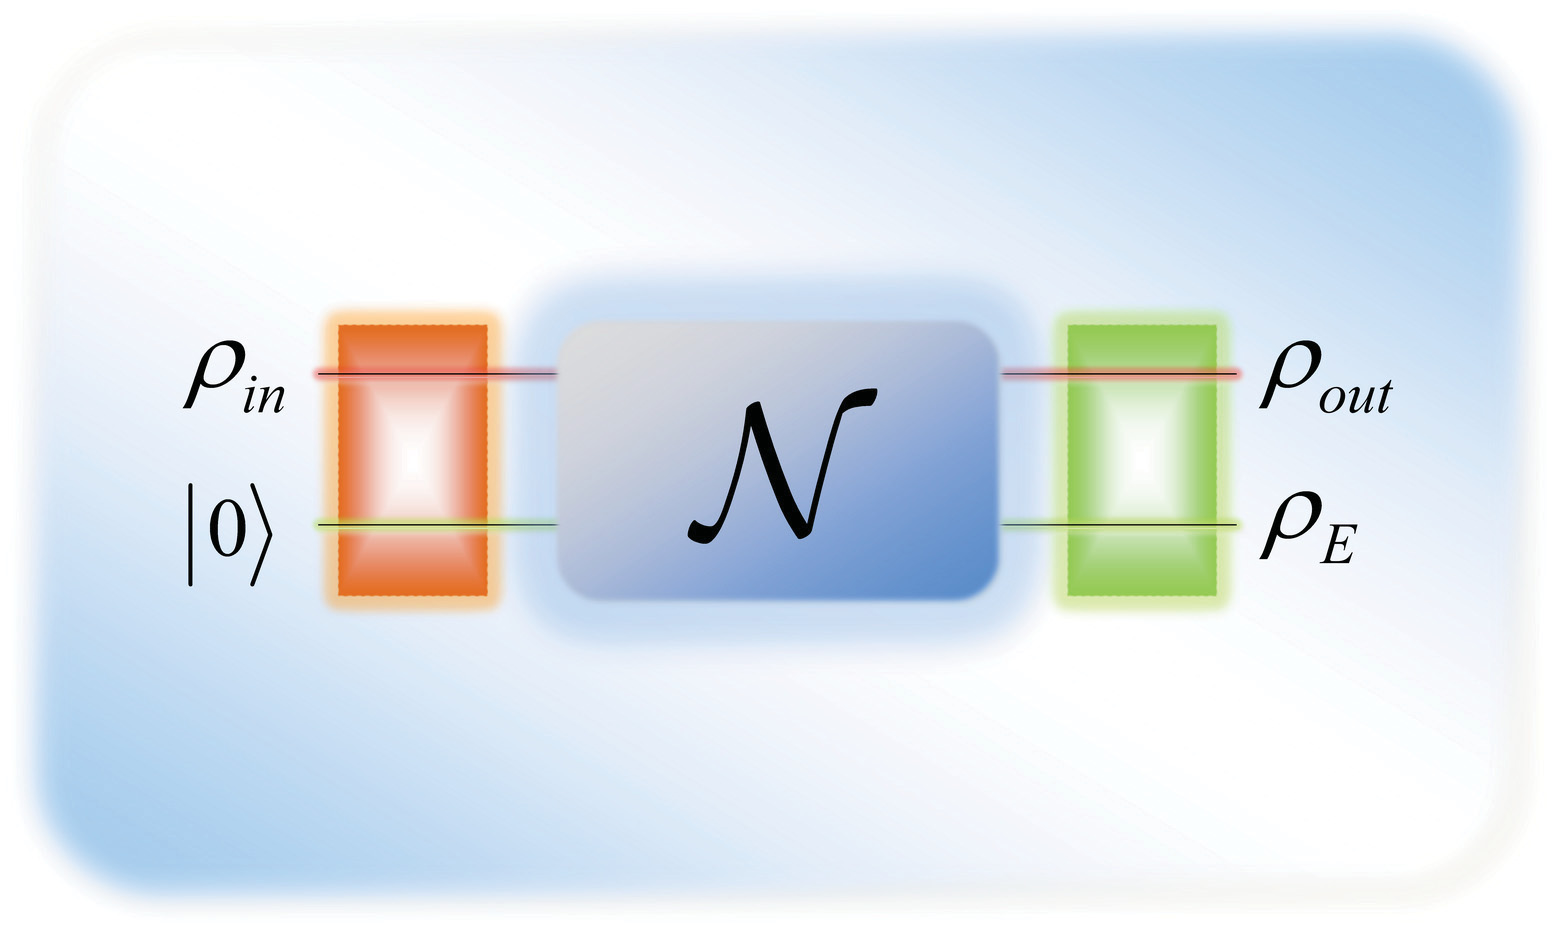
\includegraphics[scale=0.1]{channel2.png}
        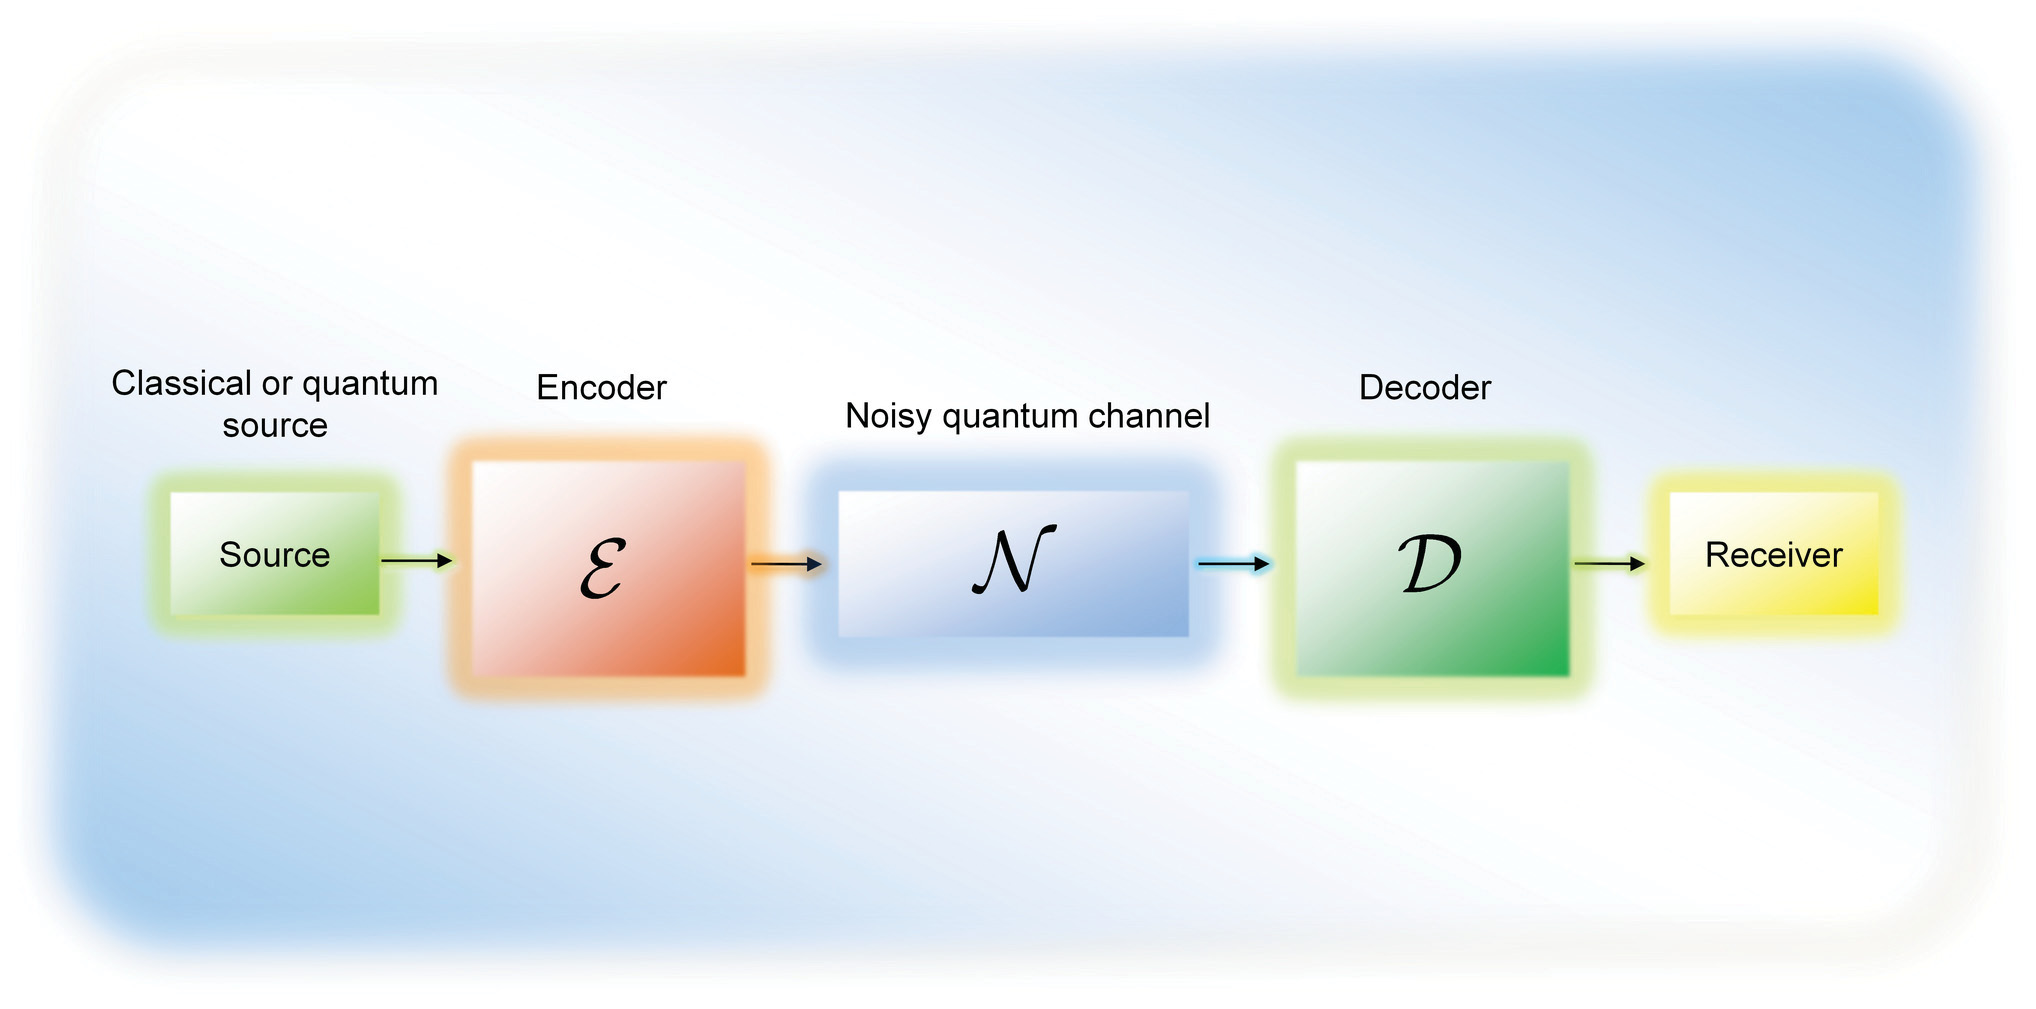
\includegraphics[scale=0.1]{channel1.png}
        \caption{Illustrations of a quantum channel \cite{Gyongyosi_2018}.}
    \end{figure}
\end{frame}

\begin{frame}{Kraus Representation}
    Quantum channels are often represented in what is called the Kraus form (or the Choi-Kraus representation). In this form, quantum channels can be defined
    as linear combination in the following way:
    \begin{equation}
        \mathcal{N}(\rho) = \sum_i K_i \rho K_i^\dagger 
    \end{equation}
    where $\sum_i K_i^\dagger K_i = \mathbb{I} $\\
    The Kraus representation is very useful in as a tool for analysing quantum channels, and makes several problens easier to solve. Kraus operators and their
    uses show up at many useful places throughout Quantum information theory. It makes channels easier to understand as well, by decomposing them into several
    "sub-channels".
\end{frame}

\begin{frame}{Von Neumann Entropy}
    The quantum analogue of the classical entropy is the Von Neumann Entropy. It is defined on the density operator as:
    \begin{equation}
        S(\rho) = -Tr[\rho log(\rho)]
    \end{equation}
    Its maximum value is for the maximally mixed state and mimimum for a pure state.\\
    Any quantum state can be spectrally decomposed to be written as $\sigma = \sum_{i}p_i | x_i \rangle \langle x_i |$ where ${x_i}$ are eigenvectors
    and ${p_i}$ are eigenvalues. Some algebraic manipulation can show that the quantum entropy ($S(\sigma)$) will be equivalent to the classical entropy of
    a probability distribution described by the eigenvalues:
    \begin{equation}
        S(\sigma) = H(p) = \sum_i p_i log(p_i)
    \end{equation}
\end{frame}

\begin{frame}{Other quantities}
    Several other quantities are defined for quantum systems analogous to the classical ones. Many of their properties are similar to their classical counterparts,
    but there are some striking exceptions as well. We define some of these here:
    \begin{itemize}
        \item Quantum Conditional Entropy
        $$S(A|B) = S(\rho_{AB}) - S(\rho_B)$$
        where $\rho_B$ is the system with $A$ traced out. Interestingly, this quantity can be negative, something which is not seen in its classical counterpart.
    \end{itemize}
\end{frame}

\begin{frame}{Other quantities}
    \begin{itemize}
        \item Quantum Mutual Information
        $$I(A:B) = S(\rho_A) + S(\rho_B) - S(\rho_{AB})$$
        Quantum mutual information has a greater upper bound (by 2 times) compared to its classical counterpart.
        \item Quantum Relative Entropy
        $$D(\rho || \sigma) = Tr[\rho (log(\rho) - log(\sigma))]$$
        This is analogous to the classical Kullback-Liebler Divergence.
    \end{itemize}
\end{frame}